\documentclass[12pt]{article}

\usepackage{multirow,tabularx}
\usepackage{pgfplots}
\usepackage{geometry}
\usepackage{graphicx}
\usepackage{soul}

\geometry{letterpaper, margin=1in}
\pgfplotsset{compat=1.18}

\begin{document}
\section*{Findings}
\subsection*{Absolute and relative optical data}

\ul{Absolute optical cross sections are consistently underestimated by Mie theory} (Table \ref{tab:absolute}). This applies to both scattering and absorption. Possible reasons for the mismatch between calculations and experimental data are:

\begin{itemize}
    \item Presence of larger, multiply charged particles in the aerosol
    \item Inaccuracy in model parameters, such as refractive index
    \item Deviation from spherical morphology in real particles
\end{itemize}

The second reason does not apply to aerosols with spherical particles, such as nigrosin. However, as seen in Table \ref{tab:absolute}, Mie still underestimates optical cross sections significantly even for nigrosin. A part of this report investigates the effect of multiply charged particles on the overall absorption cross section.

\subsection*{Enhancements and coating thickness}

Contrary to our belief, \ul{enhancements depend on core particle size when volume-equivalent coating thickness is the independent variable}. When the size of the scatterer is much larger than the wavelength of incident light (geometric optics), scattering cross section is proportional to the square of particle radius:

\begin{equation}
    C_{\mathrm{sca}}\propto \left(r_0+\Delta r\right)^2
    \label{eq:sca_xs}
\end{equation}

Normalizing Equation \ref{eq:sca_xs} by scattering cross section of a body with $\Delta r=0$ yields:

\begin{equation}
    E_{\mathrm{sca}}=\left(\frac{r_0+\Delta r}{r_0}\right)^2=\left(1+\frac{\Delta r}{r_0}\right)^2
    \label{eq:sca_enh}
\end{equation}

As seen from Equation \ref{eq:sca_enh}, scattering enhancement for a very large particle depends not only on coating thickness, but also on its initial size. Given this information, it does not make sense to assume that enhancements would be independent on core particle size in the range of Mie scattering. Numerical Mie estimates support this (Table \ref{tab:enhancements} and Figure \ref{fig:enhancements}).

On the other hand, using $\mathrm{Gfm}$ as the independent variable does cancel out the size differences of core particles when $r>>\lambda$. Particle radius can be expressed as a function of $\mathrm{Gfm}$:

\begin{equation}
    r=r_0\sqrt[3]{1+\frac{\rho_{\mathrm{core}}}{\rho_{\mathrm{shell}}}\left(\mathrm{Gfm}-1\right)}
    \label{eq:r_vs_gfm}
\end{equation}

Substituting Equation \ref{eq:r_vs_gfm} into Equation \ref{eq:sca_xs} yields:

\begin{equation}
    C_{\mathrm{sca}}\propto r_0^2\left(1+\frac{\rho_{\mathrm{core}}}{\rho_{\mathrm{shell}}}\left(\mathrm{Gfm}-1\right)\right)^\frac{2}{3}
    \label{eq:sca_xs_gfm}
\end{equation}

Finally, normalizing Equation \ref{eq:sca_xs_gfm} by scattering cross section of a body with $\mathrm{Gfm}=1$, which is proportional to $r_0^2$ according to Equation \ref{eq:sca_xs_gfm}, yields:

\begin{equation}
    E_{\mathrm{sca}}=\left(1+\frac{\rho_{\mathrm{core}}}{\rho_{\mathrm{shell}}}\left(\mathrm{Gfm}-1\right)\right)^\frac{2}{3}
    \label{eq:sca_gfm}
\end{equation}

As seen from Equation \ref{eq:sca_gfm}, scattering enhancement for a very large particle does not depend on initial particle size when expressed in terms of Gfm. The same applies to Rayleigh scattering. Although this does not necessarily generalize to Mie scattering regime, it would be a more reasonable assumption.

\subsection*{SSA and refractive indices}

\ul{Refractive indices with different imaginary parts}, such as indices of black carbon and nigrosin, \ul{cause a difference in SSA which is amplified by addition of non-absorbing coating} (Table \ref{tab:ssa} and Figure \ref{fig:ssa}).

\subsection*{Absorption of polydisprese aerosols}

\ul{Large absorbing particles significantly contribute to overall absorption cross section even if their number fraction in the aerosol is small}. Calculations have been performed for a nigrosin aerosol consisting of three particle modes: 150 nm, 236 nm, and 315 nm. Number fractions of each particle size were estimated from an SEM image of a collected sample (Figure \ref{fig:sem}).

Fractional contribution of a particle mode $i$ where $i\in [1,3]$ was estimated with the following equation:

\begin{equation}
    \mathrm{Contribution}=\frac{C_\mathrm{abs}^{(i)}\times f^{(i)}}{\sum_{n=1}^3{C_\mathrm{abs}^{(n)}\times f^{(n)}}}
\end{equation}

Even though the number fraction of triply charged particles (315 nm) was only $4\%$ in the sample, the absorption contribution of that mode is $22\%$. Absorption contribution of double charged particles (236 nm) is $29\%$.

On the other hand, \ul{MAC is not a strong function of particle size}. MAC mostly depends on the refractive index of the material and is around 4.2 $\mathrm{m}^2/\mathrm{g}$ for nigrosin. All numeric results are reported in Table \ref{tab:absorption}.

\newpage

\begin{table}[!h]
\centering
\caption{Calculated and measured optical cross sections for bare aerosols ($\mathrm{m}^2\times10^{14}$)}
\begin{tabular}{c c c c c}
    \hline
     & \multicolumn{2}{c}{Measured} & \multicolumn{2}{c}{Mie} \\
     & C\textsubscript{abs} & C\textsubscript{sca} & C\textsubscript{abs} & C\textsubscript{sca} \\
     \hline
     Nigrosin & 2.05 & 1.87 & 1.14 & 0.504 \\
     CB200\textsubscript{cmp} & 1.54 & 0.787 & 0.767 & 0.123 \\
     CB200\textsubscript{agg} & 4.20 & 2.63 & 3.09 & 1.34 \\
     BC & 2.43 & 0.833 & 1.49 & 0.398 \\
     \hline
\end{tabular}
\label{tab:absolute}
\end{table}

\begin{table}[!h]
\centering
\caption{Calculated optical cross sections ($\mathrm{m}^2\times10^{14}$) and enhancements for nigrosin particles coated with DOS}
\begin{tabular}{c c c c c c c c c}
    \hline
     \multirow{2}{*}{$\Delta r_{ve}$, nm} &  \multicolumn{4}{c}{150 nm} & \multicolumn{4}{c}{240 nm}\\
     & C\textsubscript{abs} & E\textsubscript{abs} & C\textsubscript{sca} & E\textsubscript{sca} & C\textsubscript{abs} & E\textsubscript{abs} & C\textsubscript{sca} & E\textsubscript{sca} \\
     \hline
     0 & 1.04 & 1.00 & 0.51 & 1.00 & 4.94 & 1.00 & 4.62 & 1.00 \\
     10 & 1.17 & 1.12 & 0.80 & 1.59 & 5.35 & 1.08 & 5.74 & 1.24 \\
     20 & 1.28 & 1.23 & 1.22 & 2.41 & 5.72 & 1.16 & 7.06 & 1.53 \\
     40 & 1.49 & 1.43 & 2.47 & 4.89 & 6.29 & 1.27 & 10.44 & 2.26 \\
     80 & 1.88 & 1.81 & 8.37 & 16.54 & 6.99 & 1.41 & 20.58 & 4.46 \\
     \hline
\end{tabular}
\label{tab:enhancements}
\end{table}

% SSA for different RIs
\begin{table}[!h]
    \centering
    \caption{SSA for 150 nm particles coated with DOS with $1.7+0.6i$ and $1.7+0.3i$ refractive indices}
    \begin{tabular}{c c c}
        \hline
        $\Delta r_{\mathrm{ve}},\ \mathrm{nm}$ & $1.7+0.6i$ & $1.7+0.3i$ \\
        \hline
        0 & 0.248 & 0.305 \\
        10 & 0.294 & 0.383 \\
        20 & 0.345 & 0.460 \\
        40 & 0.450 & 0.597 \\
        80 & 0.672 & 0.800 \\
        \hline
    \end{tabular}
    \label{tab:ssa}
\end{table}

\begin{table}[!h]
    \centering
    \caption{Absorption characteristics of nigrosin particles calculated with Mie. Quantitative statistics from Figure \ref{fig:sem}}
    \begin{tabular}{c c c c}
        \hline
        & 150 nm & 236 nm & 315 nm \\
        \hline
        Fraction ($f$) & 0.84 & 0.11 & 0.04 \\
        $C_{\mathrm{abs}},\ \mathrm{m}^2\times10^{14}$ & 1.04 & 4.70 & 9.64 \\
        $C_{\mathrm{abs}}\times f,\ \mathrm{m}^2\times10^{15}$ & 8.76 & 5.17 & 3.86 \\
        Contribution, $C_{\mathrm{abs}}\times f\over C_{\mathrm{abs,total}}$ & 0.493 & 0.291 & 0.217 \\
        Mass, fg & 2.49 & 9.70 & 23.08 \\
        MAC, $\mathrm{m}^2/\mathrm{g}$ & 4.19 & 4.48 & 4.18 \\
        \hline
    \end{tabular}
    \label{tab:absorption}
\end{table}

\begin{figure}[!h]
    \centering
    \resizebox{\columnwidth}{!}{
    \begin{tikzpicture}
    \begin{axis}[
    xlabel={$\Delta r_{\mathrm{ve}}$, nm},
    ylabel=$E_{\mathrm{abs}}$,
    legend pos=north west
    ]
        \addplot table [x=dr,y=E_abs_150] {pgfdata/mie.txt};
        \addlegendentry{150 nm}
        \addplot table [x=dr,y=E_abs_240] {pgfdata/mie.txt};
        \addlegendentry{240 nm}
    \end{axis}
    \end{tikzpicture}
    \begin{tikzpicture}
    \begin{axis}[
    xlabel={$\Delta r_{\mathrm{ve}}$, nm},
    ylabel=$E_{\mathrm{sca}}$
    ]
        \addplot table [x=dr,y=E_sca_150] {pgfdata/mie.txt};
        \addplot table [x=dr,y=E_sca_240] {pgfdata/mie.txt};
    \end{axis}
    \end{tikzpicture}
    }
    \caption{Absorption and scattering enhancements for nigrosin particles coated with DOS, calculated with Mie theory (Data source: Table \ref{tab:enhancements})}
    \label{fig:enhancements}
\end{figure}

\begin{figure}[!h]
    \centering
    \begin{tikzpicture}
    \begin{axis}[
    xlabel={$\Delta r_{\mathrm{ve}}$, nm},
    ylabel=$\mathrm{SSA}$,
    legend pos=north west
    ]
        \addplot table [x=dr,y=0.6i] {pgfdata/ssa.txt};
        \addlegendentry{$1.7+0.6i$}
        \addplot table [x=dr,y=0.3i] {pgfdata/ssa.txt};
        \addlegendentry{$1.7+0.3i$}
    \end{axis}
    \end{tikzpicture}
    \caption{SSA for 150 nm particles coated with DOS, calculated with Mie theory (Data source: Table \ref{tab:ssa})}
    \label{fig:ssa}
\end{figure}

% 1, 2 and 3 charges - nigrosin
\begin{figure}[!h]
    \centering
    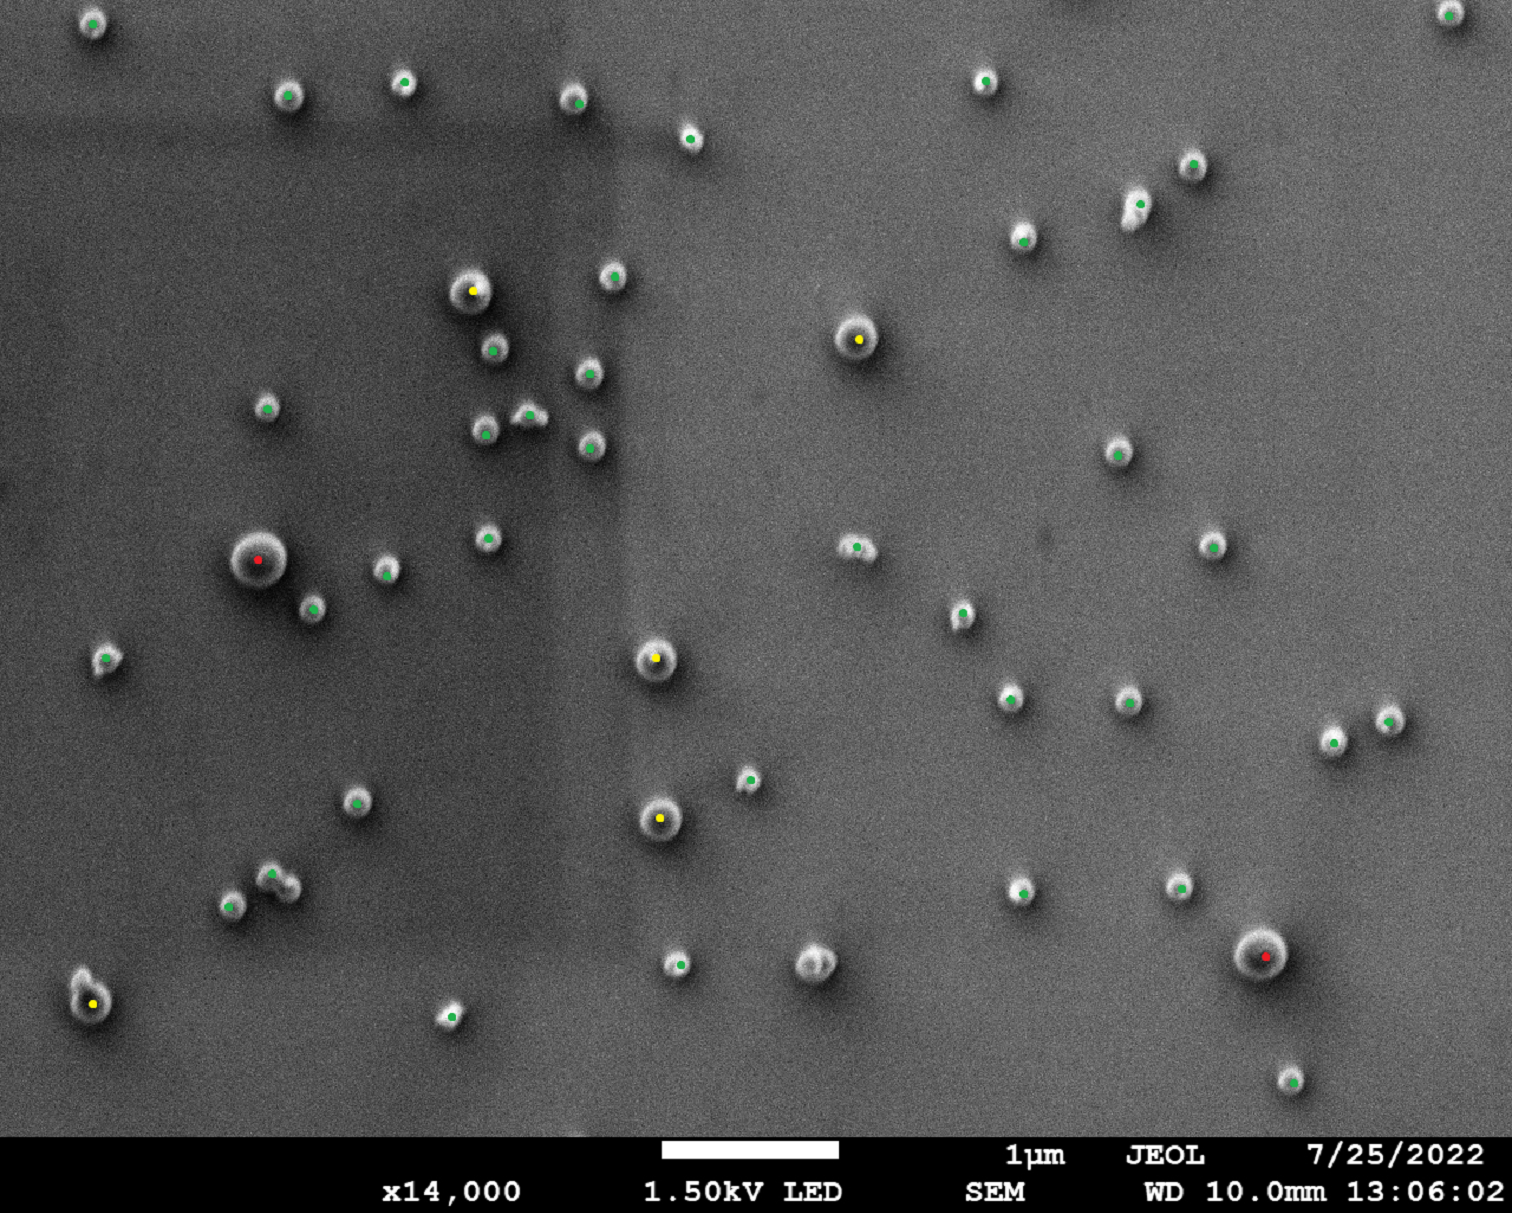
\includegraphics[width=\textwidth]{pgfdata/sem.png}
    \caption{SEM image of a 150 nm nigrosin sample. One charge (green), two charges (yellow), and three charges (red). Counts: 38 green, 5 yellow, 2 red}
    \label{fig:sem}
\end{figure}

\end{document}